% Options for packages loaded elsewhere
\PassOptionsToPackage{unicode}{hyperref}
\PassOptionsToPackage{hyphens}{url}
\PassOptionsToPackage{dvipsnames,svgnames*,x11names*}{xcolor}
%
\documentclass[
]{article}
\usepackage{lmodern}
\usepackage{amssymb,amsmath}
\usepackage{ifxetex,ifluatex}
\ifnum 0\ifxetex 1\fi\ifluatex 1\fi=0 % if pdftex
  \usepackage[T1]{fontenc}
  \usepackage[utf8]{inputenc}
  \usepackage{textcomp} % provide euro and other symbols
\else % if luatex or xetex
  \usepackage{unicode-math}
  \defaultfontfeatures{Scale=MatchLowercase}
  \defaultfontfeatures[\rmfamily]{Ligatures=TeX,Scale=1}
  \setmainfont[]{cochineal}
  \setsansfont[]{Fira Sans}
  \setmonofont[]{Fira Code}
\fi
% Use upquote if available, for straight quotes in verbatim environments
\IfFileExists{upquote.sty}{\usepackage{upquote}}{}
\IfFileExists{microtype.sty}{% use microtype if available
  \usepackage[]{microtype}
  \UseMicrotypeSet[protrusion]{basicmath} % disable protrusion for tt fonts
}{}
\makeatletter
\@ifundefined{KOMAClassName}{% if non-KOMA class
  \IfFileExists{parskip.sty}{%
    \usepackage{parskip}
  }{% else
    \setlength{\parindent}{0pt}
    \setlength{\parskip}{6pt plus 2pt minus 1pt}}
}{% if KOMA class
  \KOMAoptions{parskip=half}}
\makeatother
\usepackage{xcolor}
\IfFileExists{xurl.sty}{\usepackage{xurl}}{} % add URL line breaks if available
\IfFileExists{bookmark.sty}{\usepackage{bookmark}}{\usepackage{hyperref}}
\hypersetup{
  pdftitle={Spatial econometrics},
  colorlinks=true,
  linkcolor=Maroon,
  filecolor=Maroon,
  citecolor=Blue,
  urlcolor=blue,
  pdfcreator={LaTeX via pandoc}}
\urlstyle{same} % disable monospaced font for URLs
\usepackage[margin=1in]{geometry}
\usepackage{color}
\usepackage{fancyvrb}
\newcommand{\VerbBar}{|}
\newcommand{\VERB}{\Verb[commandchars=\\\{\}]}
\DefineVerbatimEnvironment{Highlighting}{Verbatim}{commandchars=\\\{\}}
% Add ',fontsize=\small' for more characters per line
\usepackage{framed}
\definecolor{shadecolor}{RGB}{248,248,248}
\newenvironment{Shaded}{\begin{snugshade}}{\end{snugshade}}
\newcommand{\AlertTok}[1]{\textcolor[rgb]{0.94,0.16,0.16}{#1}}
\newcommand{\AnnotationTok}[1]{\textcolor[rgb]{0.56,0.35,0.01}{\textbf{\textit{#1}}}}
\newcommand{\AttributeTok}[1]{\textcolor[rgb]{0.77,0.63,0.00}{#1}}
\newcommand{\BaseNTok}[1]{\textcolor[rgb]{0.00,0.00,0.81}{#1}}
\newcommand{\BuiltInTok}[1]{#1}
\newcommand{\CharTok}[1]{\textcolor[rgb]{0.31,0.60,0.02}{#1}}
\newcommand{\CommentTok}[1]{\textcolor[rgb]{0.56,0.35,0.01}{\textit{#1}}}
\newcommand{\CommentVarTok}[1]{\textcolor[rgb]{0.56,0.35,0.01}{\textbf{\textit{#1}}}}
\newcommand{\ConstantTok}[1]{\textcolor[rgb]{0.00,0.00,0.00}{#1}}
\newcommand{\ControlFlowTok}[1]{\textcolor[rgb]{0.13,0.29,0.53}{\textbf{#1}}}
\newcommand{\DataTypeTok}[1]{\textcolor[rgb]{0.13,0.29,0.53}{#1}}
\newcommand{\DecValTok}[1]{\textcolor[rgb]{0.00,0.00,0.81}{#1}}
\newcommand{\DocumentationTok}[1]{\textcolor[rgb]{0.56,0.35,0.01}{\textbf{\textit{#1}}}}
\newcommand{\ErrorTok}[1]{\textcolor[rgb]{0.64,0.00,0.00}{\textbf{#1}}}
\newcommand{\ExtensionTok}[1]{#1}
\newcommand{\FloatTok}[1]{\textcolor[rgb]{0.00,0.00,0.81}{#1}}
\newcommand{\FunctionTok}[1]{\textcolor[rgb]{0.00,0.00,0.00}{#1}}
\newcommand{\ImportTok}[1]{#1}
\newcommand{\InformationTok}[1]{\textcolor[rgb]{0.56,0.35,0.01}{\textbf{\textit{#1}}}}
\newcommand{\KeywordTok}[1]{\textcolor[rgb]{0.13,0.29,0.53}{\textbf{#1}}}
\newcommand{\NormalTok}[1]{#1}
\newcommand{\OperatorTok}[1]{\textcolor[rgb]{0.81,0.36,0.00}{\textbf{#1}}}
\newcommand{\OtherTok}[1]{\textcolor[rgb]{0.56,0.35,0.01}{#1}}
\newcommand{\PreprocessorTok}[1]{\textcolor[rgb]{0.56,0.35,0.01}{\textit{#1}}}
\newcommand{\RegionMarkerTok}[1]{#1}
\newcommand{\SpecialCharTok}[1]{\textcolor[rgb]{0.00,0.00,0.00}{#1}}
\newcommand{\SpecialStringTok}[1]{\textcolor[rgb]{0.31,0.60,0.02}{#1}}
\newcommand{\StringTok}[1]{\textcolor[rgb]{0.31,0.60,0.02}{#1}}
\newcommand{\VariableTok}[1]{\textcolor[rgb]{0.00,0.00,0.00}{#1}}
\newcommand{\VerbatimStringTok}[1]{\textcolor[rgb]{0.31,0.60,0.02}{#1}}
\newcommand{\WarningTok}[1]{\textcolor[rgb]{0.56,0.35,0.01}{\textbf{\textit{#1}}}}
\usepackage{graphicx}
\makeatletter
\def\maxwidth{\ifdim\Gin@nat@width>\linewidth\linewidth\else\Gin@nat@width\fi}
\def\maxheight{\ifdim\Gin@nat@height>\textheight\textheight\else\Gin@nat@height\fi}
\makeatother
% Scale images if necessary, so that they will not overflow the page
% margins by default, and it is still possible to overwrite the defaults
% using explicit options in \includegraphics[width, height, ...]{}
\setkeys{Gin}{width=\maxwidth,height=\maxheight,keepaspectratio}
% Set default figure placement to htbp
\makeatletter
\def\fps@figure{htbp}
\makeatother
\setlength{\emergencystretch}{3em} % prevent overfull lines
\providecommand{\tightlist}{%
  \setlength{\itemsep}{0pt}\setlength{\parskip}{0pt}}
\setcounter{secnumdepth}{-\maxdimen} % remove section numbering
%% See: https://bookdown.org/yihui/rmarkdown-cookbook/multi-column.html
%% I've made some additional adjustments based on my own preferences (e.g. cols
%% should be top-aligned in case of uneven vertical length)
\newenvironment{columns}[1][]{}{}

\newenvironment{column}[1]{\begin{minipage}[t]{#1}\ignorespaces}{%
\end{minipage}
\ifhmode\unskip\fi
\aftergroup\useignorespacesandallpars}

\def\useignorespacesandallpars#1\ignorespaces\fi{%
#1\fi\ignorespacesandallpars}

\makeatletter
\def\ignorespacesandallpars{%
  \@ifnextchar\par
    {\expandafter\ignorespacesandallpars\@gobble}%
    {}%
}
\makeatother

\title{Spatial econometrics}
\usepackage{etoolbox}
\makeatletter
\providecommand{\subtitle}[1]{% add subtitle to \maketitle
  \apptocmd{\@title}{\par {\large #1 \par}}{}{}
}
\makeatother
\subtitle{Lecture title}
\usepackage{authblk}
                                        \author[]{Your name}
                                                            \affil{University \textbar{} Course code}
                                            \date{}

\begin{document}
\maketitle

{
\hypersetup{linkcolor=}
\setcounter{tocdepth}{2}
\tableofcontents
}
\hypertarget{before-you-begin}{%
\subsection{Before you begin}\label{before-you-begin}}

This template is aimed at people who want to knit their R Markdown
documents to \emph{both} HTML and PDF with as few surprises as possible.
As the name suggests, I predominantly use it for my lecture notes. But I
find that it works well for writing papers too.

See the package
\href{https://github.com/grantmcdermott/lecturenotes/blob/master/README.md}{README}
for a longer description, as well as potential gotchas and limitations
(e.g.~font support for different LaTeX engines).

\hypertarget{template-features}{%
\subsection{Template features}\label{template-features}}

Here are some examples of features not available in vanilla R Markdown
and how to use them.

\hypertarget{multi-column-environments}{%
\subsubsection{Multi-column
environments}\label{multi-column-environments}}

Multi-column environments are supported via's Pandoc's
\href{https://pandoc.org/MANUAL.html\#extension-fenced_divs}{fenced\_divs}
syntax and some preamble sugar (bundled together with the template). For
example, a two-column section would look like this.

\begin{columns}[T]
\begin{columns}

\begin{column}{0.48\textwidth}
\begin{column}{0.48\textwidth}

Here is some example \textbf{dplyr} code.

\begin{Shaded}
\begin{Highlighting}[]
\KeywordTok{library}\NormalTok{(dplyr)}
\end{Highlighting}
\end{Shaded}

\begin{verbatim}
## 
## Attaching package: 'dplyr'
\end{verbatim}

\begin{verbatim}
## The following objects are masked from 'package:stats':
## 
##     filter, lag
\end{verbatim}

\begin{verbatim}
## The following objects are masked from 'package:base':
## 
##     intersect, setdiff, setequal, union
\end{verbatim}

\begin{Shaded}
\begin{Highlighting}[]
\NormalTok{mtcars }\OperatorTok\StringTok{ }
\StringTok{  }\KeywordTok{group_by}\NormalTok{(am) }\OperatorTok\StringTok{ }
\StringTok{  }\KeywordTok{summarise}\NormalTok{(}\KeywordTok{mean}\NormalTok{(mpg))    }
\end{Highlighting}
\end{Shaded}

\begin{verbatim}
## `summarise()` ungrouping output (override with `.groups` argument)
\end{verbatim}

\begin{verbatim}
## # A tibble: 2 x 2
##      am `mean(mpg)`
##   <dbl>       <dbl>
## 1     0        17.1
## 2     1        24.4
\end{verbatim}

\end{column}
\end{column}

\begin{column}{0.04\textwidth}
\begin{column}{0.04\textwidth}

~

\end{column}
\end{column}

\begin{column}{0.48\textwidth}
\begin{column}{0.48\textwidth}

And the \textbf{data.table} equivalent.

\begin{Shaded}
\begin{Highlighting}[]
\KeywordTok{library}\NormalTok{(data.table)}
\end{Highlighting}
\end{Shaded}

\begin{verbatim}
## 
## Attaching package: 'data.table'
\end{verbatim}

\begin{verbatim}
## The following objects are masked from 'package:dplyr':
## 
##     between, first, last
\end{verbatim}

\begin{Shaded}
\begin{Highlighting}[]
\NormalTok{mtcars_dt =}\StringTok{ }\KeywordTok{as.data.table}\NormalTok{(mtcars)}
\NormalTok{mtcars_dt[, }\KeywordTok{mean}\NormalTok{(mpg), by =}\StringTok{ }\NormalTok{am]   }
\end{Highlighting}
\end{Shaded}

\begin{verbatim}
##    am       V1
## 1:  1 24.39231
## 2:  0 17.14737
\end{verbatim}

\end{column}
\end{column}

\end{columns}
\end{columns}

The same idea can be extended to additional columns and the individual
column widths are also adjustable.

\hypertarget{pdf-support-for-non-standard-fonts}{%
\subsubsection{PDF support for non-standard
fonts}\label{pdf-support-for-non-standard-fonts}}

This is an easy one; simply a matter of adding \texttt{dev:\ cairo\_pdf}
to the YAML. But it's nice not having to remember that every time, no?

\emph{Note: As the figure caption suggests, to run this next chunk
you'll need to add
\href{https://docs.microsoft.com/en-us/typography/font-list/arial-narrow}{Arial
Narrow} to your font book if it's not installed on your system already.}

\begin{Shaded}
\begin{Highlighting}[]
\KeywordTok{library}\NormalTok{(ggplot2)}
\KeywordTok{library}\NormalTok{(hrbrthemes)}

\KeywordTok{ggplot}\NormalTok{(mtcars, }\KeywordTok{aes}\NormalTok{(mpg, wt)) }\OperatorTok{+}
\StringTok{  }\KeywordTok{geom_point}\NormalTok{() }\OperatorTok{+}
\StringTok{  }\KeywordTok{labs}\NormalTok{(}\DataTypeTok{x=}\StringTok{"Fuel efficiency (mpg)"}\NormalTok{, }\DataTypeTok{y=}\StringTok{"Weight (tons)"}\NormalTok{,}
       \DataTypeTok{title=}\StringTok{"This plot uses Arial Narrow fonts"}\NormalTok{,}
       \DataTypeTok{caption=}\StringTok{"Note: Fonts must be installed separately on your system."}\NormalTok{) }\OperatorTok{+}\StringTok{ }
\StringTok{  }\KeywordTok{theme_ipsum}\NormalTok{()}
\end{Highlighting}
\end{Shaded}

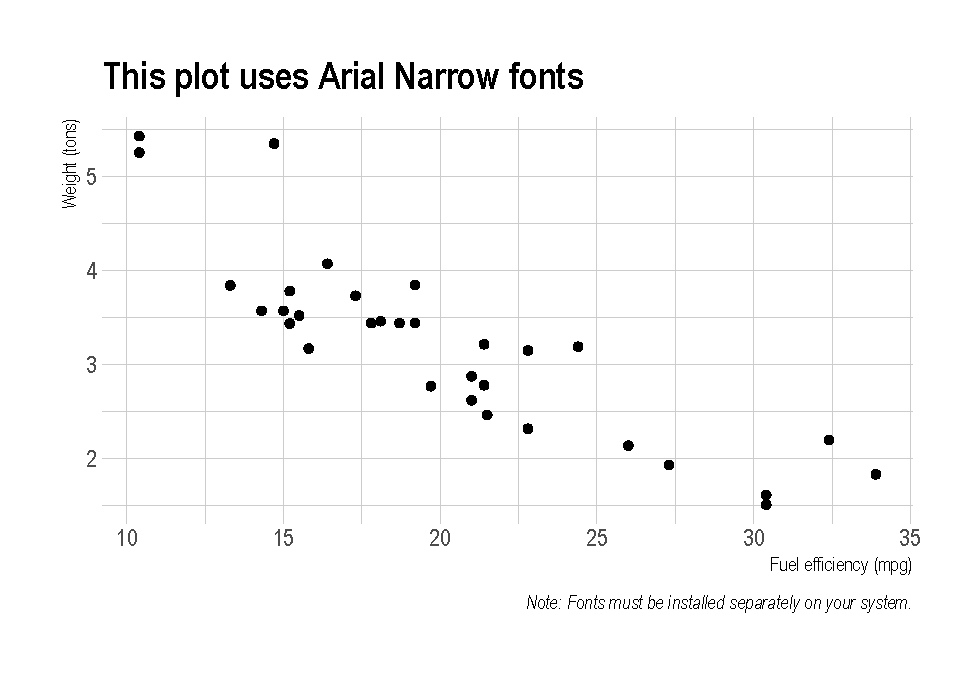
\includegraphics{ESDA-notes_files/figure-latex/mpg-1.pdf}

\hypertarget{ignore-interactive-content-when-exporting-to-pdf}{%
\subsubsection{Ignore interactive content when exporting to
PDF}\label{ignore-interactive-content-when-exporting-to-pdf}}

In general, this template tries to do a good job of automatically
handling (i.e.~ignoring) interactive content when exporting to PDF. A
notable exception is with embedded interactive content like external
GIFs. In this case, rather than typing the usual, say,
\texttt{!{[}{]}(mind-blown.gif)} directly in the Rmd file, you should
include the figure with \texttt{knitr::include\_graphics} in an R chunk.
This will allow you to control whether it renders, conditional on output
format. For example, the following chunk will render an actual GIF when
the knit target is HTML format, versus a message when that target is PDF
format.

\begin{verbatim}
## Sorry, this GIF is only available in the the HTML version of the notes.
\end{verbatim}

\end{document}
